XML is a textual markup language in which data elements are ordered by nature: \textit{string} is the core data type, other data types like integers, floats, user-defined abstract data, etc. are derived. ~\citep{xmark/original}. It is both human and machine readable, and  used as the data exchange format in the web. XML is derived from Standard Generalized Markup Language(SGML) and standardized by the World wide web Consortium(W3C).
\par
%JSON is a programming language model that consist of minimal textual representation and a subset of JavaScript. its web services. As it is the subset of JavaScript, it is perfectly suited 
    JSON is another data format that is designed to exchange the data in key/value format. As subset of JavaScript, it perfectly suits for the web-based services. In modern browsers parsing JSON is comparatively much faster than XML. A JSON document consists of two data structures:
\begin{itemize}
	\item Object, an unordered collection of key/value pair that are encapsulated with curly braces (\{ \}). The key is a string embedded in double quotes and followed by a column(:) to its value. The key must be unique for each object.
	%TODO:   which are numbers of key value pairs
	\item Arrays, that are an ordered list of values
\end{itemize}
A JSON value can be Object, Array, number, string, true, false and null.
  %XML is suitable for document description, that is the hierarichal elements can also have attributes, which is not available in JSON. JSON is much preferred for text format object serialization, because of its concise syntax for defining the lists of elements. An additional library is required for XML to work with JavaScript. Whereas JSON can directly parse and work directly with js objects.
  
\section{Problem to translate from XML to JSON}
JSON and XML are conceptually similar as they both are text based markups, that are designed to represent data in human-readable form, exchangeable across multiple platforms and parsable by common programming language, but differ in their syntax~\citep{lee2011jxon}. JSON and XML are fundamentally incompatible with each other, as listed below:
\begin{description}
\item[Root node and anonymous values] \hfill \\
Each XML document has one root node. JSON supports anonymous values also referred as string values, that do not need key/value pairs. For example, in Table~\ref{tbl:Anonymous-xmljson} the XML root node is implicitly created in the model and will not have a textual representation in JSON.

	\item[Arrays] \hfill \\
		Arrays are native data types of JSON that does not exists in XML. There is no direct markup for arrays in XML.
		\item[Identifiers] \hfill \\
		XML is much more restrictive for identifiers compared to JSON, which allows any string to be an identifier. Translating from XML to JSON does not cause any problem, but in reverse case it might lead to not well formed XML. For example, "Hello World" is a valid identifier in JSON but not valid attribute or element in XML, as there is a whitespace between the two words.
		\item[Attributes] \hfill \\
		JSON does not have the notion or any representation of attributes. When mapping data from XML to JSON, the attributes are translated to name object members along with other child elements. This information will be lost in mapping from JSON to XML.
		\item[Namespaces] \hfill \\
		XML supports namespaces to identify  unique element and attributes in a document. Namespaces do not exist in JSON. Mapping QNames in XML with namespaces to JSON can lead to ambiguous and duplicate names.
		%\item \textit{Others}\\
		%TODO: {Processing Instructions, Character Set, Comments, Encodings}
		%There are also some other problems like processing instructions and  comments which XML supports but not in JSON. Other issues for example, character set and encoding are not easily exchangeable in both format.
\end{description}

\begin{longtable}{c|c}
	\caption{Anonymous values of JSON in XML}
	\label{tbl:Anonymous-xmljson}\\
	\textbf{JSON} & \textbf{XML}\\
	\hline
\begin{minipage}{.35\textwidth}
\begin{fakeJSON}[basicstyle=\scriptsize]
	["Hello World"]
\end{fakeJSON}	
\end{minipage} &
\begin{minipage}{.45\textwidth}
\begin{fakeXML}[label=xml-anonymous]
	<root>Hello World</root>
\end{fakeXML}
or
\begin{fakeXML}
	<root value="Hello World">
\end{fakeXML}
\end{minipage}\\
\end{longtable}
	
	
		
\section{Mapping}
XML and JSON have different data types. XML has more flexible data types compare with JSON. Table~\ref{tbl:xml-json:types} types of data are listed for simple XML and relevant JSON types.
\begin{longtable}[hbtp]{c|c}
\caption{Translation of simple XML data types into JSON}
\label{tbl:xml-json:types}\\

\textbf{XML type definition} & \textbf{JSON type definition}\\
\hline

\begin{minipage}{.4\textwidth}
  \begin{lstlisting}
xs:string
  \end{lstlisting}
\end{minipage} &
\begin{minipage}{.4\textwidth}
\begin{lstlisting}
{
  "type": "string"
}
\end{lstlisting}
\end{minipage}\\

\hline
\begin{minipage}{.4\textwidth}
  \begin{lstlisting}
xs:boolean
  \end{lstlisting}
\end{minipage} &
\begin{minipage}{.4\textwidth}
\begin{lstlisting}
{
  "type": "boolean"
}
\end{lstlisting}
\end{minipage}\\

\hline
\begin{minipage}{.4\textwidth}
  \begin{lstlisting}
xs:float
xs:double
xs:decimal
xs:integer
(All Other Numbers)
  \end{lstlisting}
\end{minipage} &
\begin{minipage}{.4\textwidth}
\begin{lstlisting}
{
  "type": "number"
}
\end{lstlisting}
\end{minipage}\\
\hline

\begin{minipage}{.4\textwidth}
	\begin{lstlisting}
xs:anySimpleType
(Remaining all others)
	\end{lstlisting}
\end{minipage} &
\begin{minipage}{.4\textwidth}
\begin{lstlisting}
{
	"type": "string"
}
\end{lstlisting}
\end{minipage}\\
\end{longtable}


For complex type elements in XML that contains nested elements and attributes, JSON can have two possibilities: either an object or an array type.  Sectio~\ref{xml-to-json-migration} illustrates the translation of complex XML type to JSON.

\section{Migration from XML to JSON}\label{xml-to-json-migration}
We have defined the several stages to convert XML to JSON documents:
\begin{enumerate}[label=\textbf{Step \arabic *.}]
	\item~\\
	\textbf{XML to JSON friendly XML}
	\par
	Algorithm~\ref{algorithm-JSONXML} provides pseudo-code for XML-to-JSON friendly XML. At the first step of the conversion process, all attributes of XML document are represented as ordered child elements. There can be more than one attribute that is inserted in order. Then, the inserted attributes are deleted.  XML nodes can contain both text and element node as a child, whereas JSON can have only key/value pair or value only for array. Each text node that  has also an element node as sibling is moved to \textit{childtext}(name of the element) node. At the end of the first step, if an element contains another element as a child node, then it is represented as object type of JSON. It is necessary to identify if a siblings of an element node($S$) has same the element name or not. If this condition exists, $S$ is represented as an array in JSON. All the child nodes of all siblings are moved inside $S$ node. If $S$ is already  object type  then it is replace with array type  a new array is added. %In this algorithm, the loop of one action affect other, so they are looped independently.
	
	\item~\\
	\textbf{Data type of XML-to-JSON data type}
	\par
	After JSON-friendly XML in Step 1, the complex data type of XML is marked as either object or array type of JSON illustrated in Table~\ref{tbl:xmljson}. In this Step,  as in 
	Algorithm~\ref{algorithm-JSONXML-type}, all the scalar type of XML document are identified and marked with their type in JSON according to Table ~\ref{tbl:xml-json:types}.
	\item~\\
	\textbf{Mapping XML to JSON object or array}
	\par
	After Step 1 and 2, a complete JSON-friendly XML is generated. All XML objects and arrays are mapped to $<$$key$, $value$$>$ pair of JSON and their respective data types. Table ~\ref{tbl:xmljson-convert-3} illustrates final conversion from XML to JSON.
\end{enumerate}

		\begin{algorithm}[h]
			\DontPrintSemicolon
        	\begin{algorithmic}
        	\STATE Initialize $D = "{XML} document"$;
        	  	\FORALL{descendant-or-self node of  $D$,  $X$ which has attributes $A$  }
        			\STATE move  all attributes  $A$ to ordered child element of $X$\;
        		\ENDFOR
        		
        		\FORALL{descendant-or-self node of  $D$,$X$ }
        			\IF{ $X$ contains Text node and element node Both}
        				\STATE create new element "childtext" \;
        				\STATE move text node to "childtext" element \;
        			\ENDIF
        		\ENDFOR
        		
        		\FORALL{descendant node of  $D$,$X$ }
        			\FORALL{child element $C$ in $X$}
        				\IF{ $C$ has siblings $S$ with same \textit{name} }
        					\STATE convert $C$ as Array type\;
        					\STATE move child of $S$ into $C$ as $<$\_$>$ element\;
        				\ENDIF
        				\IF{ $C$ has child element }
        					\STATE convert $C$ as Object type\;
        				\ENDIF
        			\ENDFOR
        		\ENDFOR
        	\end{algorithmic}
        	\caption{Pseudocode to convert normal  XML to JSON friendly XML}\label{algorithm-JSONXML}
\end{algorithm}
	
 \begin{algorithm}[h]
			\DontPrintSemicolon
        	\begin{algorithmic}
        	\STATE Initialize $D = "{XML} document"$;
        	  	\FORALL{descendant-or-self node of  $D$ as $C$}
        			\IF{ $C$ has no attribute "type" }
        				\STATE get content of $C$ \;
                        \STATE identify content type according to Table ~\ref{tbl:xml-json:types}. and add attribute to $C$ "type" \;
        			\ENDIF
        		\ENDFOR
        	\end{algorithmic}
        	\caption{ convert data type of XML to JSON data type(Step 2)}\label{algorithm-JSONXML-type}
        \end{algorithm}

\begin{longtable}{c|c}
	\caption{XML to JSON friendly XML(step 1)}
	\label{tbl:xmljson}\\
	\textbf{XML} & \textbf{ Algorithm~\ref{algorithm-JSONXML} }\\
	\hline
\begin{minipage}{.4\textwidth}
\begin{fakeXML}
<info>
  <name>
    <f>a</f>
  </name>
  <age>24</age>
  <ismarried>false</ismarried>
  <city name="Armonk"/>
  <state>NY</state>
  <contact>
	 home
    <p>993-330</p>
    <p>993-331</p>
  </contact>
</info>
\end{fakeXML}	
\end{minipage} &
\begin{minipage}{.55\textwidth}
\begin{fakeXML}
<info type="object">
  <name type="object">
    <f>a</f>
  </name>
  <age>24</age>
  <ismarried>false</ismarried>
  <city type="object">
    <name>Armonk</name>
  </city>
  <state>NY</state>
  <contact type="object">
	<childtext>home</childtext>
    <p  type="array" >
	   <_>993330</_>
	   <_>993-331</_>
    </p>
  </contact>
</info>
\end{fakeXML}
\end{minipage}\\
\end{longtable}

\begin{longtable}{c|c}
	\caption{XML to JSON friendly XML(step 2)}
	\label{tbl:xmljson-2}\\
	\textbf{Algorithm~\ref{algorithm-JSONXML}} & \textbf{ Algorithm~\ref{algorithm-JSONXML-type} }\\
	\hline
\begin{minipage}{.4\textwidth}
\begin{fakeXML}
<info type="object">
  <name type="object">
    <f>a</f>
  </name>
  <age>24</age>
  <ismarried>false</ismarried>
  <city type="object">
    <name>Armonk</name>
  </city>
  <state>NY</state>
  <contact type="object">
	 <childtext>home</childtext>
    <p  type="array" >
	   <_>993330</_>
	   <_>993-331</_>
    </p>
  </contact>
</info>
\end{fakeXML}	
\end{minipage} &
\begin{minipage}{.55\textwidth}
\begin{fakeXML}
<info type="object">
  <name type="object">
    <f type="string">a</f>
  </name>
  <age type="number">24</age>
  <ismarried type="boolean">false</ismarried>
  <city type="object">
    <name type="string">Armonk</name>
  </city>
  <state>NY</state>
  <contact type="object">
	 <childtext type="string">home</childtext>
    <p  type="array" >
	   <_ type="number">993330</_>
	   <_ type="string">993-331</_>
    </p>
  </contact>
</info>
\end{fakeXML}
\end{minipage}\\
\end{longtable}

	\begin{longtable}{c|c}
	\caption{XML to JSON (step 3.)}
	\label{tbl:xmljson-convert-3}\\
	\textbf{XML(After step 2)} & \textbf{JSON}\\
	\hline
\begin{minipage}{.55\textwidth}
\begin{fakeXML}
<info type="object">
  <name type="object">
    <f type="string">a</f>
  </name>
  <age type="number">24</age>
  <ismarried type="boolean">false</ismarried>
  <city type="object">
    <name type="string">Armonk</name>
  </city>
  <state type="string">NY</state>
  <contact type="object">
	<childtext type="string">home</childtext>
    <p  type="array" >
	   <_ type="number">993330</_>
	   <_ type="string">993-331</_>
    </p>
  </contact>
</info>
\end{fakeXML}	
\end{minipage} &
\begin{minipage}{.5\textwidth}
\begin{fakeJSON}
{
    "info":{
      "name":{
        "f":"a"
      },
      "age":24,
      "ismarried":false,
      "city":{
        "name":"Armonk"
      },
      "state":"NY",
      "contact":{
	   "childtext":"home",
        "p":[
          993330,
          "993-331"
        ]
      }
    }
}
\end{fakeJSON}
\end{minipage}\\
\end{longtable}
	
\section{XMark}\label{xmark}
			The XML benchmarking project XMARK~\citep{xmark/original} is one of the most popular and commonly used XML benchmarking projects to date. It provides a small executable tool called \textit{xmlgen} that can be used to create a synthetic XML dataset based on a fixed schema describing an Internet auctions database. xmlgen can be used to build a single record with a large, hierarchical XML tree structure. A factor is specified to scale the generated data, ranging from a few kilobytes to an arbitrary size, limited by the capacity of the system. The textual part of the resulting XML document is constructed from 17,000 most frequently occurring words of Shakespeare's plays.

\subsection{Dataset}\label{xmark-dataset}
The main entities of XMark data are in two groups. The first group consists of  \textit{person}, \textit{open\_auction}, \textit{closed\_auction}, \textit{item} and \textit{category}. The second group's entities \textit{annotation} and \textit{description} are natural language text and document-centric element structure. The relationship between the entities in the first group are expressed as reference and the second group entities are embedded into subtree of first group entities. Figure~\ref{fig:xmark-tree} shows the XMark dataset with the following properties:
\label{xmark:desc:each}
\begin{itemize}	
	\item
	\textit{people} is a collection of \textit{person} element that is connected to buyer and seller of \textit{open\_auctions}, \textit{closed\_auctions}, etc. Each person has an unique identifier \textit{id} to reference to another entities like open\_auctions and closed\_auctions.
	\item
	\textit{regions} is a collection world regions \textit{africa}, \textit{asia}, \textit{australia}, \textit{europe}, \textit{namerica} and \textit{samerica}. Each of these region has \textit{item} elements which are the objects for sale or already sold. Each \textit{item} carries a unique identifier \textit{id} and has properties like name, payment information, description and a reference to the seller that are encoded as elements. 
	\item
		\textit{open\_auctions} refers to current auctions that contains bid history(increase/decrease over time) with references to bidders and sellers, current bid, the time interval of bid accepted, the status of the transaction, a reference to the item being sold etc.
	\item
		\textit{closed\_auctions} contains auctions that are successfully completed. They have properties like buyer and seller information reference to \textit{person}, a reference to sold items, amount of price, quantity of sold items, date of transaction, type of transaction, and much more.
	\item 
		\textit{categories} is used to classify the items. Each category has a unique identifier used to reference an item, a name and a description.
	\item
		  A \textit{catgraph} links categories into a network.  The full semantics of the XMark dataset can be found in~\cite{xmark/original}.
\end{itemize}
The full ER-Diagram of XMark dataset is illustrated in Fig.~\ref{fig:xmark-schema}. 
\begin{figure}[H]
	\centering
	\subfloat[Reference in \textit{XMark}]{
		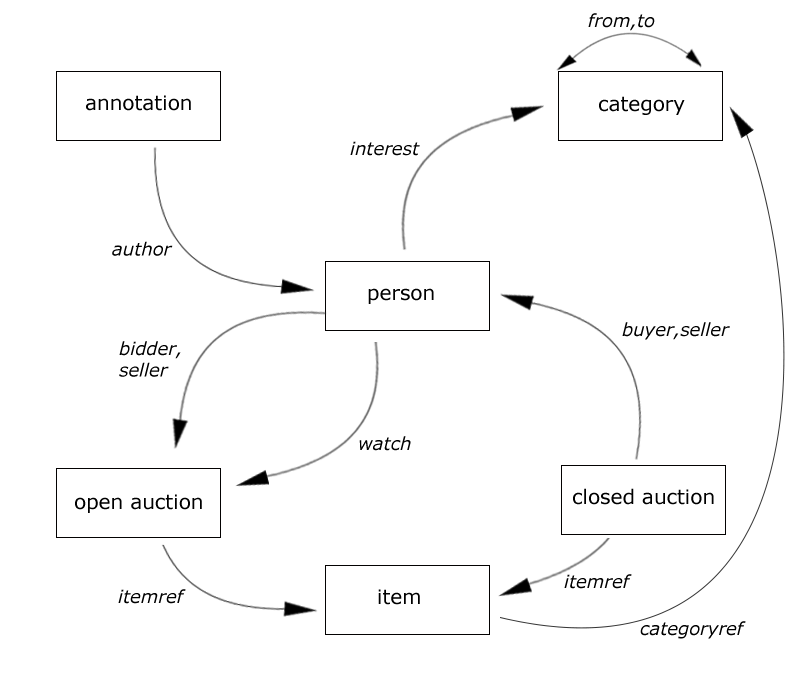
\includegraphics[width=0.40\textwidth]{img/xmark/101}{ %xmark-references.png
			\label{fig:xmark-reference}
		}
	}
	\centering
	\subfloat[Reference in \textit{XMark} dataset tree]{
		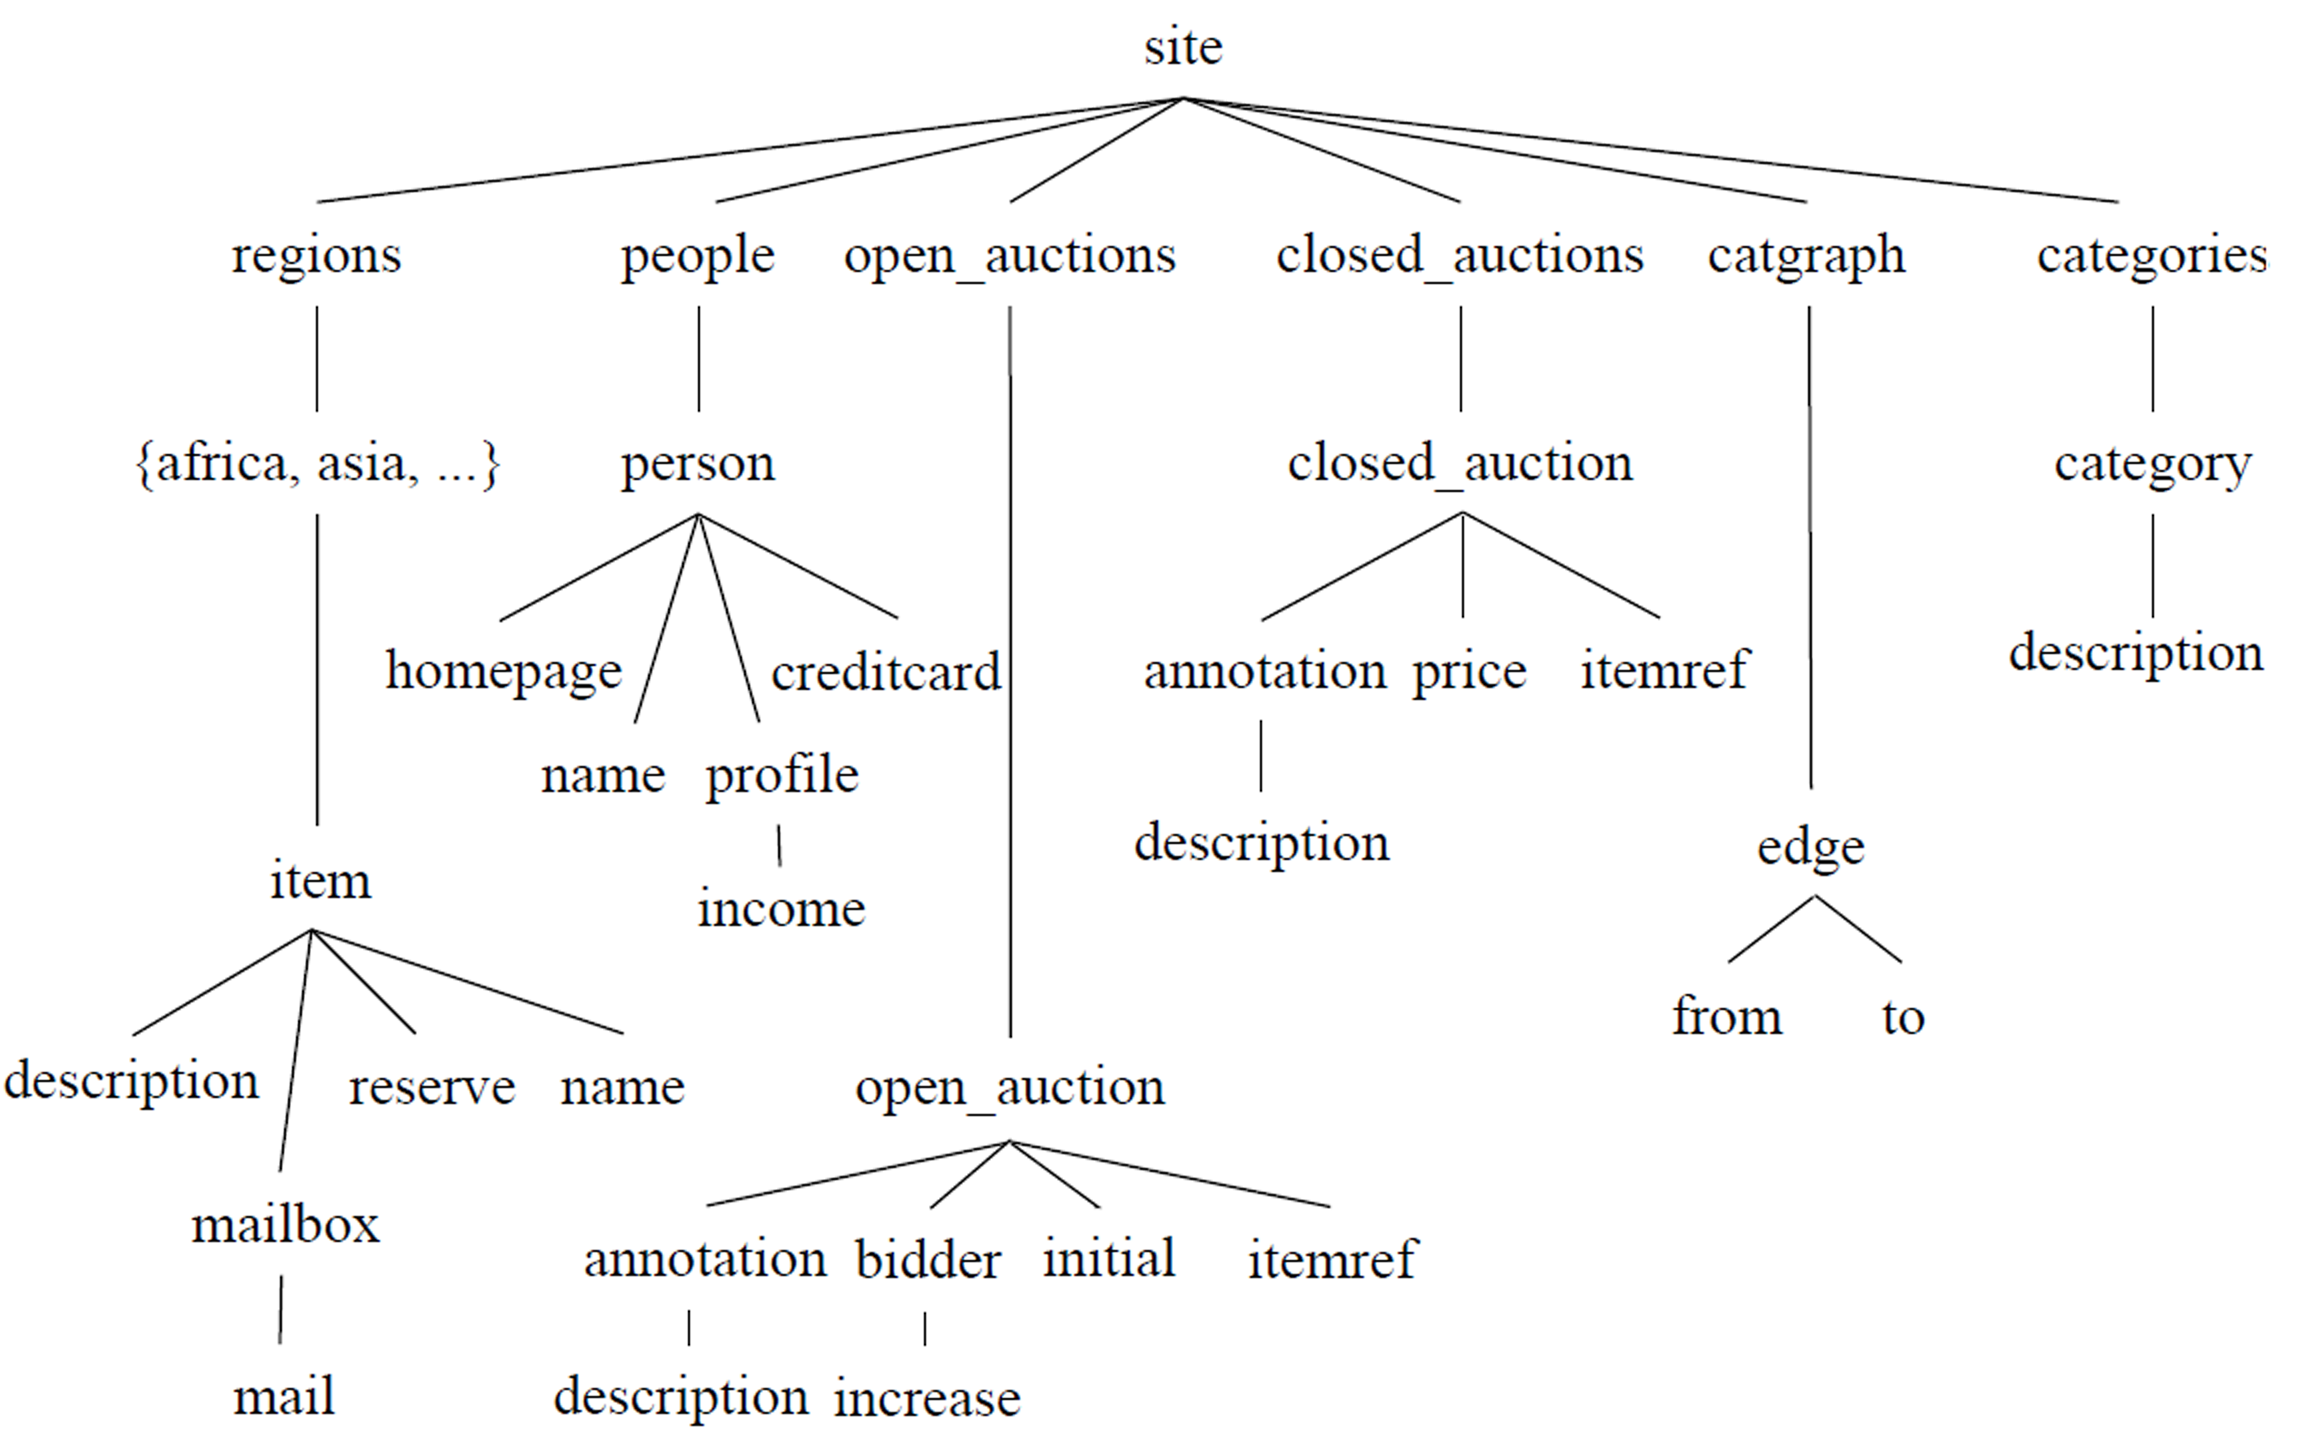
\includegraphics[width=0.4\textwidth]{img/xmark-tree.png}{
			\label{fig:xmark-tree}
		}
	}
	\caption{XMark data tree and reference~\citep{xmark/original}}
	\label{fig:xmark-tree-reference}
\end{figure}
\begin{figure}[H]
	\centering
	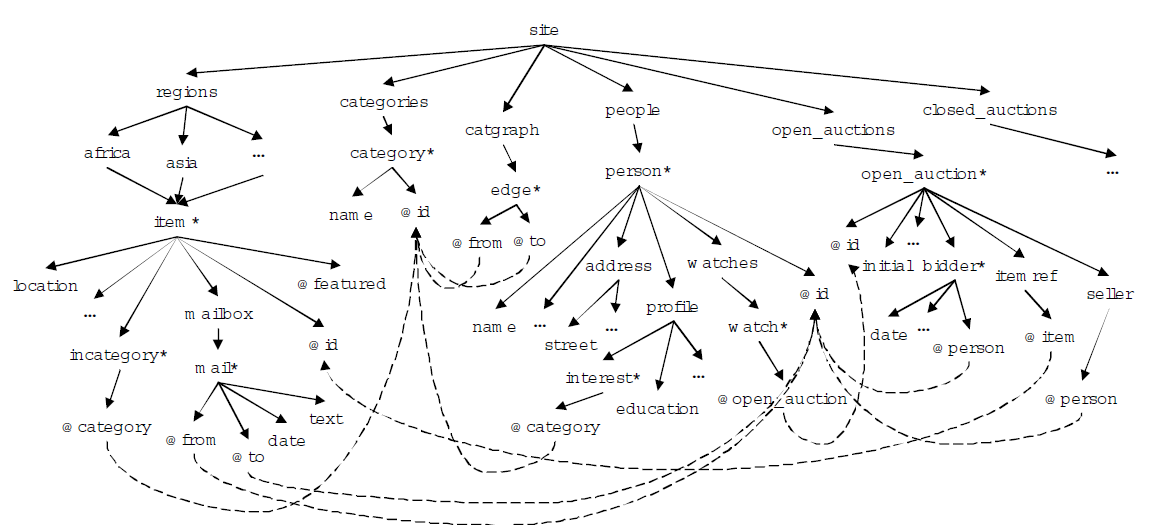
\includegraphics[width=0.90\textwidth]{img/xmark-schema-4}
	\caption{XMark ER-Diagram. Nodes, solid arrows, and dashed arrows represent schema elements (or attributes, with prefix '@'), structural links, and value links, respectively. Elements with suffix '*' are of SetOf type\citep{xmark/schema-sumerize}}
	\label{fig:xmark-schema}
\end{figure}

\subsection{XMark Queries}\label{xmark-queries}
The XMark project contains XQuery queries that focuses on the various aspect of language such as aggregation, reference, ordering, wildcard expressions, joins, user defined functions, etc.\citep{xmark/mlynkova2008xml}.The textual representation of 20 different XQuery expressions is reprinted in  Table~\ref{tab:xmark-queries}. These queries are divided into different categories  based on the  multiple functionalities of XQuery: 
\begin{enumerate}[label=\arabic*.]
\item  First category tests execution of exact match of string in specified path and consists of only query Q1.
\item It  helps to analyze order access of an XML document. Query Q2, Q3 and Q4 are grouped here.
\item  Query Q5 is evaluates the casting of a value.
\item Queries Q6 and Q7  evaluate regular path expressions.

\item This category investigates the referencing of a document to another and consists of query Q8 and Q9

\item Query Q10 reconstructs a complex results from the result of a query

\item Two queries, Q11 and Q12 are join query based on values.  The difference between this category's queries and reference queries Q8 and Q9 is that references are specified in DTD and may optimize with object identifiers whereas Q11 and Q12 are have join on the basis of values.

\item Query Q13  benchmarks the portion reconstruction of original XML document.

\item In this category the full text search  using single word is implemented. Q14 is in this category

\item The purpose of queries 15 and 16 is to observe the path traversals without using wildcards.

\item Query Q17 tests the ability to deal with missing values

\item This category deals with user defined functions and contains query Q18

\item The query Q19 is use to evaluate Sorting.

\item The last category observe the aggregation with the help of query 20.

\end{enumerate}

\begin {table}[htpb] 
\centering
\caption {The XMark queries. Source:\citep{xmark/original}}
\label {tab:xmark-queries}
\begin{tabular}{r|l}
	\hline
	Q1&Return the name of the person with ID 'person0'.\\
	\hline
	Q2&Return the initial increase of all open auctions.\\
	\hline
	Q3&Return the first and current increase of all open auctions whose current\\
	&increase is at least twice as high as the initial increase.\\
	\hline
	Q4&List the reserves of those open auctions where a certain person issued\\
	&a bid before another person.\\
	\hline
	Q5&How many sold items cost more than 40.\\
	\hline
	Q6&How many items are listed on all continents?\\
	\hline
	Q7&How many pieces of prose are in our database?\\
	\hline
	Q8&List the names of persons and the number of items they bought.\\
	&(Joins person, closed\_auction)\\
	\hline
	Q9&List the names of persons and the names of items they bought in Europe.\\
	&(Joins person\_auction, item)\\
	\hline
	Q10&List all persons according to their interest; use French markup\\
	&in the result.\\
	\hline
	Q11&For each person, list the number of items currently on sale whose\\
	&price does not exceed 0.02\% of the person's income.\\
	\hline
	Q12&For each richer-than-average person, list the number of items currently\\
	&on sale whose price does not exceed 0.02\% of the person's income.\\
	\hline
	Q13&List the names of items registered in Australia along with\\
	&their description.\\
	\hline
	Q14&Return the names of all items whose description contains the word 'gold'.\\
	\hline
	Q15&Print the keywords in emphasis in annotations of closed auctions.\\
	\hline
	Q16&Return the IDs of those auctions that have one or more keywords\\
	&in emphasis.\\
	\hline
	Q17&Which persons don't have a homepage?\\
	\hline
	Q18&Convert the currency of the reserve of all open auctions to\\
	&another currency.\\
	\hline
	Q19&Give an alphabetically ordered list of all items along with their location.\\
	\hline
	Q20&Group customers by their income and output the cardinality of each\\
	&group.\\
	\hline
\end{tabular}
\end {table}

		\subsection{XMark data into NoSQL database}\label{xmark-nosql}
			A synthetic XMARK dataset consists of a huge record in tree structure~\citep{xmark/VIST}. As mentioned in Section~\ref{xmark-dataset}, each subtree, \textit{regions}, \textit{people}, \textit{open\_auctions}, \textit{closed\_auctions}, \textit{catgraph} and \textit{categories} contain large numbers of instances that are indexed during database creation. At first, in most NoSQL database, the dataset cannot be a huge block but in fragmented form with each instances having it's own index structure. Besides this, NoSQL databases limits the size of a single document. For example, MongoDB has a limitation of 16 MB per document, the maximum size of documents allowed in RethinkDB is 64 MB and Couchbase Server can have value of a key upto 20 MB. The data model of NoSQL does not match single instance model of XML database.
\par 
To model XMark dataset into NoSQL, we have broken down the tree structure of XMark into set of sub-structure without losing the overall data. Each NoSQL database has their own data model, hence it is required to define a model for each of those databases separately.

The generalized concept of  XMark data into NoSQL databases is explained here but it might slightly differ from one another. 

All sub-trees \textit{regions}, \textit{people}, \textit{open\_auctions}, \textit{closed\_auctions}, \textit{catgraph} and \textit{categories} are the basic unit for the document fragmentation. Each of these sub-trees stores entities \textit{item}, \textit{person}, \textit{open\_auction}, \textit{closed\_auction} and \textit{category} respectively as mentioned in Section~\ref{xmark-dataset}. These entities represent the documents in NoSQL databases. In each document, one special field \textit{doctype} is added to represent the name of parent sub-tree. For example, in case of \textit{people} sub-tree, the value of \textit{doctype} is \textit{people}. This key/value set will be the part of a document as  given in Table~\ref{tbl:xmark-xml-json}(b). The \textit{doctype} has all-together six distinct values : \textit{categories}, \textit{catgraph}, \textit{people}, \textit{open\_auctions} and \textit{closed\_auctions}. There is an exceptional case for \textit{item} entities. It has \textit{regions} as grandparent and name of different regions like \textit{asia}, \textit{europe}, \textit{australia}, \textit{namerica}, \textit{samerica} etc. as the parent.  The \textit{doctype} for \textit{item} document will be \textit{regions} as other. To represent the name of regions like \textit{asia}, \textit{europe}, etc.,  one field with key \textit{regions} is added in each document. 
Table~\ref{tbl:xmark-item-type} illustrate the extra attribute added in each of document.

\begin{longtable}{c|c}
	\caption{ Extra attribute of a document in NoSQL}
	\label{tbl:xmark-item-type}\\
    {for \textit{person} and all other entities except \textit{item} } & {for \textit{item} which has region name \textit{asia}}\\
	\hline
\begin{minipage}{.4\textwidth}
\begin{lstlisting}[language=JSON]
{
	"doctype":"people"
}
\end{lstlisting}
\end{minipage} &
\begin{minipage}{.4\textwidth}
\begin{lstlisting}[language=JSON]
{
	"doctype":"regions",
	"regions":"asia"
}
\end{lstlisting}
\end{minipage}
\end{longtable}

A sample document of NoSQL database along with respective XMark document is illustrated in  Table~\ref{tbl:xmark-xml-json}. The conversion from XML to JSON is carried out using algorithms of Section~\ref{xml-to-json-migration} with one extra attribute "doctype" to represent the parent of a document. If an element in XML has siblings with same name, they are represented as an array in NoSQL document which is already mentioned in algorithm~\ref{algorithm-JSONXML}. As it can be seen, the \textit{person} of XMark is a document in NoSQL, it is not necessary to represent this attribute.  

\begin{longtable}{c|c}
	\caption{Example: XMARK data with id \textit{person0} in XML and JSON format }
	\label{tbl:xmark-xml-json}\\
	{\textit{person0}} in XML(a) & {\textit{person0}} in JSON for a NoSQL database(b)\\
	\hline
	\begin{minipage}{.4\textwidth}
\centering		
\begin{lstlisting}[language=XML,basicstyle = \tiny,label=code:xml-nosql-person0]
<people>
    <person id="person0">
       <name>Kasidit Treweek</name>
       <emailaddress>mailto:Treweek@cohera.com</emailaddress>
       <phone>+0 (645) 43954155</phone>
       <homepage>http://www.cohera.com/~Treweek</homepage>
       <creditcard>9941 9701 2489 4716</creditcard>
       <profile income="20186.59">
          <interest category="category251" />
          <interest category="category341"/>
          <education>Graduate School</education>
          <business>No</business>
       </profile>
    </person>
</people>
\end{lstlisting}	
	\end{minipage} &
	\begin{minipage}{.55\textwidth}
		\centering
		\begin{lstlisting}[language=JSON, basicstyle =\tiny, label=code:json-nosql-person0, numberstyle=\tiny]
{
	"id": "person0",
	<@\textit{"doctype": "people",}@>
	"name": "Kasidit Treweek",
	"emailaddress": "mailto:Treweek@cohera.com",
	"phone": "+0 (645) 43954155",
	"homepage": "http://www.cohera.com/~Treweek",
	"creditcard": "9941 9701 2489 4716",
	"profile": {
		"income": 20186.59,
		<@\textcolor{red}{
		"interest": [{
			"category": "category251"
		},{
			"category": "category341"
		}]}@>,
		"education": "Graduate School",
		"business": "No"
	}
}
		\end{lstlisting}
	\end{minipage}\\
\end{longtable}



\begin{comment}
\iffalse\fi
\begin{minipage}{.5\textwidth}
	\begin{tikzpicture}[%
	grow via three points={one child at (0.5,-0.7) and
		two children at (0.5,-0.7) and (0.5,-1.4)},
	edge from parent path={(\tikzparentnode.south) |- (\tikzchildnode.west)}]
	\node {\{asfdasfd\}}
	child { node [defi] {\textit{Schema\_ID}}}
	child { node [json] {xs:attribute}
		child { node [defi] {\textit{Attribute\_ID}}}
		child { node [attribute] {@name}}
		child { node [attribute] {@type}}
		child { node [attribute] {@fixed}}
		child { node [attribute] {@default}}
	};
	\end{tikzpicture}
\end{minipage}

\end{comment}


			\subsubsection{XMARK dataset in MongoDB}\label{xmark-mongodb}
				In MongoDB, collections consist of group of documents with similar structure. Therefore, the data modeling concept of Section~\ref{xmark-nosql} has to be modified marginally. The documents are grouped with their \textit{doctype} from Section~\ref{xmark-nosql}. Each \textit{doctype} represent a collection, there are all together 6 collections. The field \textit{doctype} is already represented as collections, it is removed from all documents.  
For \textit{item} entity,  field \textit{regions} does not change. The \textit{\_id} is the primary index of a document in MongoDB, the identifier attribute of the XMark data \textit{id} is renamed to \textit{\_id} for default indexing.  \textit{closed\_auctions} and \textit{catgraph} do not have an identifier attribute \textit{id}, therefore, system will automatically generate the \textit{\_id} in these collections.
A typical example of MongoDB document for person with identifier \textit{person0} is given in Figure~\ref{code:mongodb-person0}.	

\begin{figure}[hbt]
\begin{lstlisting}[language=JSON, basicstyle =\scriptsize]
    {
    	<@\textbf{"\_id": "person0",}@>
    	"name": "Kasidit Treweek",
    	"emailaddress": "mailto:Treweek@cohera.com",
    	"phone": "+0 (645) 43954155",
    	"homepage": "http://www.cohera.com/~Treweek",
    	"creditcard": "9941 9701 2489 4716",
    	"profile": {
    		"income": 20186.59,
    		"interest": [
    			{"category": "category251"},
    			{"category": "category341"}
    			],
    		"education": "Graduate School",
    		"business": "No"
    	}
    }
\end{lstlisting}
\caption{MongoDB document of XMark data in \textit{people} collection}
\label{code:mongodb-person0}
\end{figure}
			\subsubsection{XMARK dataset in Couchbase}\label{xmark-couchbase}
				\begin{figure}[h]
\begin{lstlisting}[language=JSON,  basicstyle =\scriptsize]
{
	"id":  "item1000",
	"doctype":  "regions",
	"regions":  "africa",
	"name":  "duteous nine eighteen" ,
	"payment":  "Creditcard" ,
	"quantity": 1 ,
	"shipping":  "Will ship internationally, See description for charges" ,
	"incategory": [
		{
		"category":  "category0"
		}
	] ,
	"mailbox":[],
	"description":{ }
}
\end{lstlisting} 
\caption{Couchbase pseudo-document of the XMark data for item with id \textit{item1000}}
\label{code:couchbase-item0}
\end{figure}

Couchbase does not have the concept of grouping documents like \textit{collections} in MongoDB  or \textit{tables} in RethinkDB. 
Therefore, the data model of Section ~\ref{xmark-nosql} is applied without modification.
 All the documents are stored in a single bucket with identifier attribute \textit{id} as a document key. An \textit{id} will be manually generated for the documents without identifier.
 An example of Couchbase document is illustrated in Figure~\ref{code:couchbase-item0}

			\subsubsection{XMARK dataset in Rethinkdb}\label{xmark-rethinkdb}
				RethinkDB stores the documents inside a table which is identical to the collection in MongoDB. 
The documents are grouped according to their \textit{doctype} and store in a table.
Each \textit{doctype} of \ref{xmark-nosql} is represented as an individual table. 
The tables \textit{regions}, \textit{people}, \textit{open\_auctions}, \textit{closed\_auctions}, \textit{catgraph} and \textit{categories} contains the respective documents as of \textit{doctype}. Hence the attribute \textit{doctype} is removed from all documents.  \textit{id} is the primary key and any document without \textit{id} field is automatically added as an identifier during the time of insertion. Figure~\ref{code:rethindb-person0} shows a document with id \textit{person0} in \textit{people} table.


\newbox\rethinkdbXmarkDocument
\begin{lrbox}{\rethinkdbXmarkDocument}
\begin{lstlisting}[language=JSON,basicstyle =\scriptsize]

	{
		 <@\textbf{"id": "person0"}@>,
		"name": "Kasidit Treweek",
		"emailaddress": "mailto:Treweek@cohera.com",
		"phone": "+0 (645) 43954155",
		"homepage": "http://www.cohera.com/~Treweek",
		"creditcard": "9941 9701 2489 4716",
		"profile": {
			"income": 20186.59,
			"interest": [
			    { "category": "category251" },
				{"category": "category341"}
			],
			"education": "Graduate School",
			"business": "No"
		}
	}
\end{lstlisting}
\end{lrbox}


\newbox\rethinkdbXmarkChart
\begin{lrbox}{\rethinkdbXmarkChart}
\begin{tikzpicture}[grow'=right,level distance=1.25in,sibling distance=.25in, font=\scriptsize]
\tikzset{edge from parent/.style= 
            {thick, draw, edge from parent fork right},
         every tree node/.style=
            {draw,minimum width=1in,text width=1in,align=center}}
\Tree 
    [. Database 
        [.{regions}
            [.{... } ]
        ]
        [.people
            [.{person0 } ]
        ] 
        [.{open\_auctions}
            [.{... } ]
        ]
        [.{closed\_auctions}
            [.{... } ]
        ]
        [.{catgraph}
            [.{... } ]
        ]
        [.{categories}
            [.{... } ]
        ]
    ]
    
\end{tikzpicture}
\end{lrbox}

\begin{figure}[hhtp]
\centering
\subfloat[Database, tables and documents in RethinkDB] {
    \usebox\rethinkdbXmarkChart
    \label{xmark-rethinkdb-tree}
}
\\
\centering
\subfloat[RethinkDB document \textit{person0} in \textit{people} table ] {
        \usebox\rethinkdbXmarkDocument
        \label{code:rethindb-person0}
}

\caption{XMark data in RethinkDB}
\label{xmark-rethinkdb-figure}
\end{figure}